\documentclass[12pt]{article}
\usepackage[utf8]{inputenc}
\usepackage{graphicx}
\usepackage[document]{ragged2e}
\renewcommand*\contentsname{Sommaire}

\begin{document}
\begin{titlepage}
\begin{center}
   \vspace*{1cm}
    \textbf{Rapport Intelligence Artificielle}
    \vspace{0.5cm}
   
    \vspace{1.5cm}
   
    \texttt{Terral Naomie}\\
    \texttt{Rodriguez Charlotte}\\
    \texttt{Geshkovski Borjan}
    \vfill
    
    \vspace{0.8cm}
    
   Université de Bordeaux\\
   Mai 2016
\end{center}
\end{titlepage}
\title{}
\tableofcontents
\clearpage

\section{Introduction à l'intelligence artificielle}

\subsection{L'intelligence artificielle et ses enjeux}
\justify
L'intelligence artificielle est un domaine de l'informatique consacré au dévelo-ppement de programmes, permettant aux ordinateurs d'avoir un comportement que l'on peut caractériser d'intelligent. La majeur partie de la recherche en intelligence artificielle est focalisée sur des applications extrêmement préci-ses, telles que la prise de décision, la perception, l'adaptation à un nouvel environnement, la mémoire... 
\justify
Un des buts principaux de l'intelligence artificielle est de construire des entités intelligentes autonomes, capable d'exécuter des tâches complexes à la portée de l'être humain ou non. 
\justify
Dans la communauté informatique, on observe des divergences d'opinions, quant aux objectifs de l'intelligence artificielle. 
\begin{itemize}
\item Doit-elle avoir seulement l'apparence de l'intelligence? (Intelligence artificielle forte)
\item Son fonctionnement interne doit-il être semblable à celui de l'être humain, et être au moins aussi rationnel ? (Intelligence artificielle faible)
\end{itemize}
Dans le cadre de ce projet, nous nous situons plutôt dans le domaine de l'intelligence artificielle faible, en cherchant à reproduire le mécanisme de la prise de décision de l'être humain. 
\justify
L'intelligence artificielle s'est illustrée, au cours du temps dans différentes applications. On a pu observer des utilisations de l'intelligence artificielle dans les jeux de stratégie (nécessitant une prise de décision). 
\justify
Un des événements les plus marquants des ces 30 dernières années, est la victoire de Deep Blue (superordinateur conçu par IBM), sur le champion du monde d'échec des années 90, Garry Kasparov. On se rappelle aussi de la victoire de Watson (aussi conçu par IBM), au jeu télévisé Jeopardy!, en 2011. Encore plus récemment, en 2015, le logiciel AlphaGo, créé par Google a battu le triple champion européen de jeu de Go.
\justify
Une autre application intéressante est le développement de chatbots, comme est l'exemple d'ELIZA, codé par Joseph Weizenbaum dans les années 60. Elle simule un dialogue actif entre un psychothérapeute (ordinateur) et son patient(utilisateur). C'est un intelligence artificielle, au sens de l'intelligence artificielle faible, puisqu'elle ne comprend pas ce que l'interlocuteur lui dit, et ses réponses sont construites à partir de modèles pré-établis et de mots clés identifiés dans l'entrée de l'utilisateur.
\justify
Il y a quelques mois, Microsoft a subit un lourd échec avec le chatbot Taytweets, un compte Twitter simulant le langage d'une jeune adulte de 19 ans, dans le but d'apprendre à interagir avec les utilisateurs de ce réseaux social.
\justify 
Quels sont les enjeux de l'intelligence artificielle ? 



\subsection{Le problème}
\justify
Dans ce rapport nous tendons d'aborder la question de la prise de décision, élément central à l'intelligence artificielle. Nous abordons cette problématique, selon trois points de vue différents : celui d'un agent autonome, celui d'un consommateur, et celui d'une entreprise. 
\justify
Avant de poursuivre plus, définissons les notions d'agent et de prise de décision.
\justify
Un agent est " une entité autonome, ca pable de percevoir son environnement grâce à des capteurs, et aussi d'agir sur celui-ci via des effecteurs afin de réaliser des buts. Un agent peut également apprendre et utiliser des connaissances pour pouvoir réaliser ses objectifs"\footnote{Stuart Russel et Peter Norvige, Intelligence Artificielle, 2012}.
\justify
Dans ce projet, l'agent est un aspirateur plus ou moins intelligent (il ne disposera pas obligatoirement de capteurs). Nous étudions trois classes d'aspirat-eurs : 
\begin{itemize}
\item Un aspirateur aléatoire
\item Un aspirateur disposant d'une base de règle, associée à la possibilité d'apprentissage
\item Un aspirateur dit "génétique", dont le comportement est déterminé par un algorithme d'optimisation (algorithme génétique)
\end{itemize}
On entend par prise de décisions le processus qui consiste à faire un choix parmi plusieurs alternatives.
Dans le dictionnaire, une prise de décision est définie comme un processus cognitif complexe consistant en un choix d'action parmi plusieurs alternatives. 
\justify
Au cours de ce travail nous nous concentrons sur la prise de décision (choix d'action entre aspiration ou déplacement) de ces différents types d'aspirateurs, en fonctionne leurs capteurs et leur environnement. On regardera aussi les choix fait par les entreprises et les consommateurs. 
\section{Etudes comparative}
Le monde dans lequel les agents evoluent est une sorte de damier: il est compose de n $\times$ m cases (on note n le nombre de lignes et m le nombre de colonnes), dans lesquelles peut se trouver l'agent, et / ou differents objets (qui varient en fonction de l'agent considere). L'aspirateur se trouve forcement dans une et une seule des cases du monde.
De la facon dont nous avons implementee aspirateurs et mondes, l'agent ne peut se deplacer qu'en colonne et le monde ne contient qu'une ligne.  
\subsection{Point de vue de l'agent artificielle }
\justify
La performance des agents v0 et v1 peut etre observee de deux points de vue differents : via la fonction \texttt{getEvaluation} et via la fonction \texttt{perfGlobale}. \texttt{getEvaluation} est construite de la facon suivante : (card(pieces netoyees)+1)/(card(base de connaissances)+1). Quant a \texttt{perfGlobale}, elle est implementee de la facon suivante : card (pieces nettoyees) - card (pieces visitees 3 fois ou plus). 
\justify
Les valeurs observees ne sont pas directement les resultats de ces 2 fonctions (\texttt{getEvaluation} et \texttt{perfGlobale}), mais la moyenne de ces resultats effectuee a partir de 10 simulations (sur chaque monde). 
\justify
La duree d'une simulation sur un monde est $2*$(taille du monde). 
\justify
\textbf{Aspirateur v0 (Stochy)}
\justify
Le premier agent que nous allons observer choisit une action qu'il va faire de maniere aleatoire. Il ne dispose pas des capteurs (donc le monde n'est pas observable). Les actions dont il dispose sont: \texttt{'Gauche'} (aller a gauche), \texttt{'Droite'} (aller a droite) et \texttt{'Aspirer'}.
\justify 
En plus de l'agent, les cases du monde correspondant peuvent contenir soit rien (qu'on note '.'), soit de la poussiere (qu'on note 'x'). Si l'agent choisit une action impossible a effectuer, le monde ignore cette action et reste dans l'etat dans lequel il etait avant le choix de cette action. Par exemple, si on est dans le cas de dimension $1 \times 2$ et si l'agent se trouve dans la deuxieme colonne du monde et qu'il choisit l'action \texttt{Droite}, le monde ne change pas d'etat. 
\begin{center}
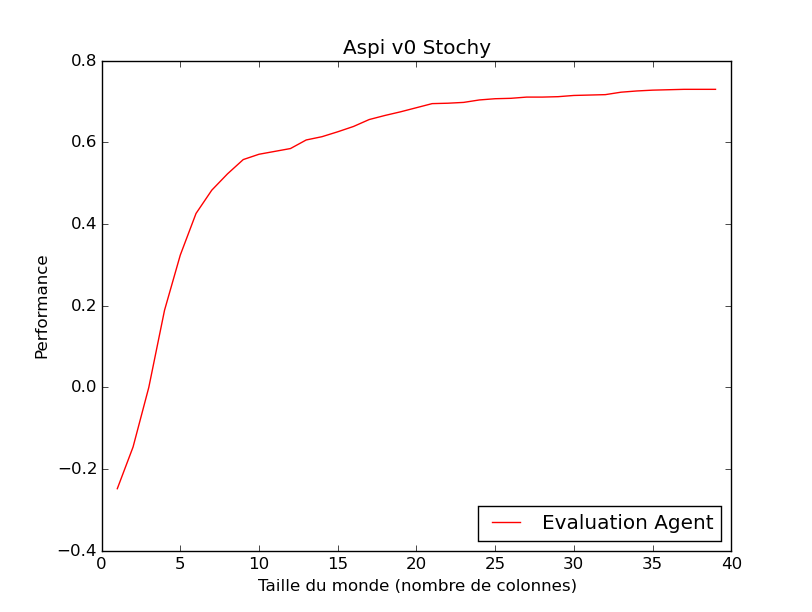
\includegraphics[scale=0.65]{figure_1}
\end{center}
\justify
Nous avons observee la performance de "Stochy" en fonction de la taille du monde. Il n'y a pas d'interet a regarder l'evaluation de \texttt{getEvaluation}, puisque l'agent a d'autant plus de chance de nettoyer un grand nombre de poussiere que la taille de monde augmente (cette taille etant proportionelle au nombre de "poussieres" presentes). On observe 

\justify
\textbf{Aspirateur v0a (Deter)}
\justify
C'est un aspirateur qui dispose de capteurs lui permettant de voir les cases du monde situees a sa position et/ou a sa gauche et/ou a sa droite. Il dispose aussi d'une base de connaissances, qui constitue des regles lui dictant des actions qu'il peut effectuer en fonction des informations qu'il recoit via ses capteurs. La base de connaissances est fixe. "Deter" va exploiter ses regles avec une probabilite qui lui est donnee (en parametre): la probabilite d'exploitiation notee $P_e$. Dans une situation donnee, il va utiliser les regles avec une probabilite $P_e$ et choisir une action d'une maniere aleatoire avec une probabilite $1-P_e$. 
\justify
\textbf{Aspirateur v1 (Learny)}
\justify
"Learny" est identique a "Deter", a l'exception du fait qu'il peut modifier la base de connaissances, c'est a dire, il dispose de la capacite d'apprendre de nouvelles regles. Au debut de la simulation, la base de connaissances peut etre vide ou non. De meme que pour "Deter", "Learny" a une probabilite d'exploitation $P_e$.
\begin{center}
\includegraphics[scale=0.65]{figure_2}
\end{center}
\justify
L'evaluation que recoit l'agent a une 

\begin{center}
\includegraphics[scale=0.65]{figure_3}
\end{center}

\justify

\justify
\textbf{Aspirateur v2 (Super Deter)}
\subsection{Point de vue de l'entreprise commerciale}
\subsection{Point de vue du consommateur}
\justify
Le consommateur doit prendre deux décisions avant d'acheter un aspirateur. Il doit tout d'abord se demander quel est la catégorie d'aspirateur le mieux adapter selon l'environnement qu'il doit aspirer, puis le consommateur doit choisir à quelle entreprise il va l'acheter. 
\begin{center}
	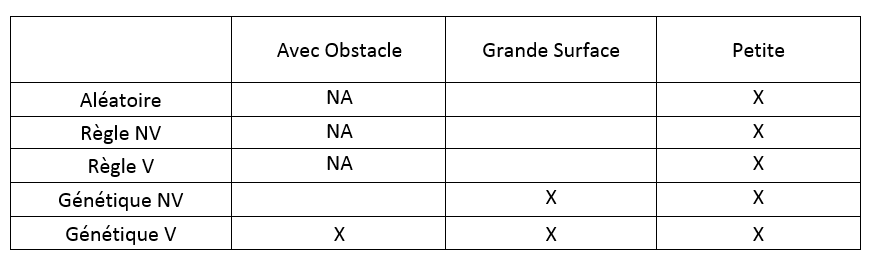
\includegraphics[scale=0.85]{Consom1}
\end{center}
\begin{center}
	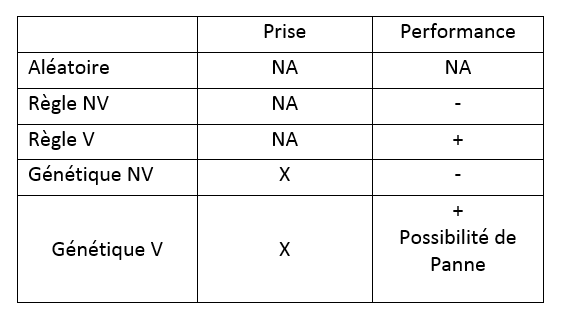
\includegraphics[scale=0.85]{Consom2}
\end{center}
\begin{center}
	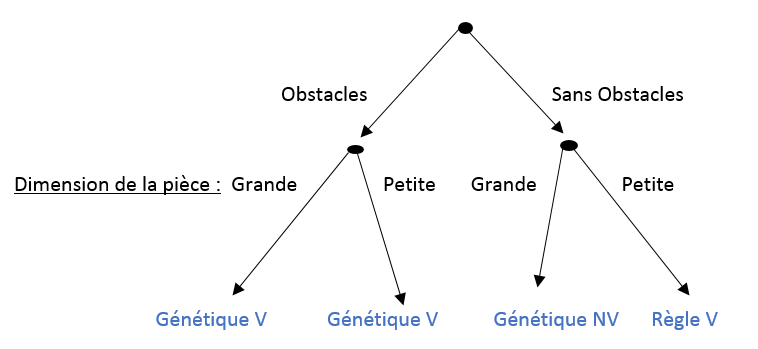
\includegraphics[scale=0.85]{Consom3}
\end{center}

\section{Intelligence d'un agent artificiel ? }

\section{Conclusion}
\end{document}